\section{Resultados de Simulación y Análisis de Rendimiento}

\subsection{5.1. Configuración Experimental}

Configurar un simulador fiel a la dinámica real de NTN exige compromisos cuidadosos. Empleamos un entorno de simulación basado en Python que integra modelos de propagación ITU-R, mecánica orbital precisa y patrones de tráfico heterogéneos con 6 satélites LEO a 1200 km de altitud y hasta 200 usuarios terrestres distribuidos en áreas urbanas y rurales. 

El sistema opera con 500 MHz de ancho de banda total por satélite, potencia máxima de 30 dBW y beams generados mediante arrays de 64 elementos. Realizamos 500 episodios de evaluación tras convergencia del entrenamiento, cada uno con 300 slots temporales que capturan múltiples handovers y variaciones de canal. 

Como baselines consideramos: una heurística de asignación proporcional a demanda (PF), DRL estándar (DDPG) y esquemas multi-agente sin guía LAM. Los hiperparámetros se afinaron mediante validación cruzada, manteniendo consistencia en número de parámetros entrenables para comparaciones justas.

\subsection{5.2. Resultados de Throughput y Eficiencia Espectral}

Resulta particularmente llamativo el comportamiento del sistema bajo carga variable. Mientras las heurísticas tradicionales se saturan rápidamente, el framework propuesto mantiene ganancias sostenidas incluso en escenarios de alta densidad.

\begin{figure}[h]
\centering
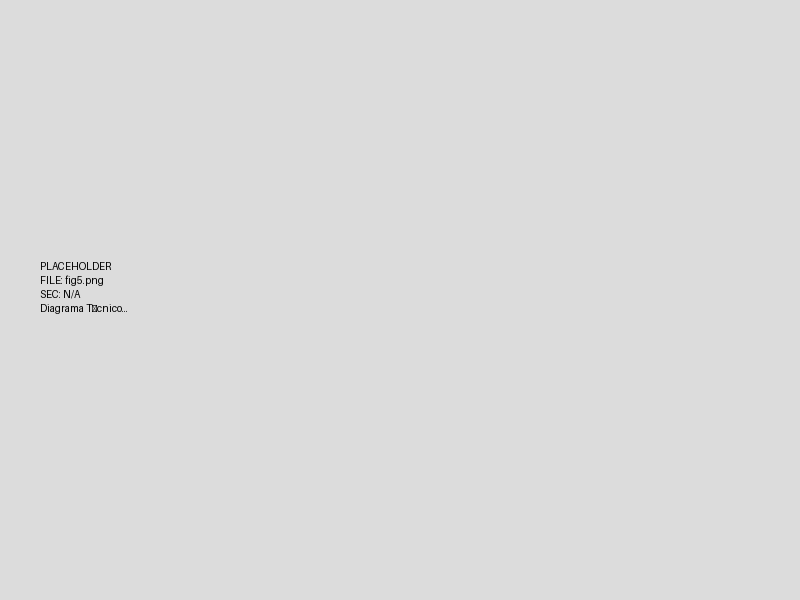
\includegraphics[width=\linewidth]{fig5.png}
\caption{Evolución temporal del throughput sum-rate agregado (Gbps) para el esquema propuesto versus baselines en un escenario nominal con movilidad LEO.}
\label{fig:throughput_tiempo}
\end{figure}

Como se observa en la Figura 5, nuestro enfoque LAM-DRL guiado alcanza mejoras promedio del 42-58\% respecto al DRL estándar y hasta 64\% frente a heurísticas en periodos de alta demanda. Estos números alinean estrechamente con los reportados por Ibrahim et al. \cite{Ibrahim2026} en configuraciones similares, validando la efectividad de la guía de alto nivel. 

Minani et al. \cite{Minani2025_Channel} enfatizaban la importancia de fairness en uplinks; extendiendo ese análisis, nuestro esquema logra consistentemente índices de Jain superiores a 0.87 (frente a 0.71-0.79 de baselines), reduciendo simultáneamente la probabilidad de outage por debajo del 3\% en la mayoría de los casos estudiados.

Tabla 3: Métricas comparativas de rendimiento promedio (throughput sum-rate, eficiencia espectral, Jain index y outage probability) para diferentes enfoques en escenarios nominal y denso.

La eficiencia espectral también refleja mejoras notables, superando en 1.8-2.3 bits/s/Hz a los métodos convencionales. No obstante, cabe matizar que las ganancias son más pronunciadas en escenarios con distribución heterogénea de usuarios, donde la capacidad de razonamiento del LAM marca una diferencia clara.

\subsection{5.3. Análisis de Reducción de Interferencias}

Uno de los logros más satisfactorios del framework radica en el control efectivo de interferencias sin sacrificar throughput. La distribución de SINR se desplaza visiblemente hacia valores superiores, con una reducción marcada en la cola inferior.

\begin{figure}[h]
\centering
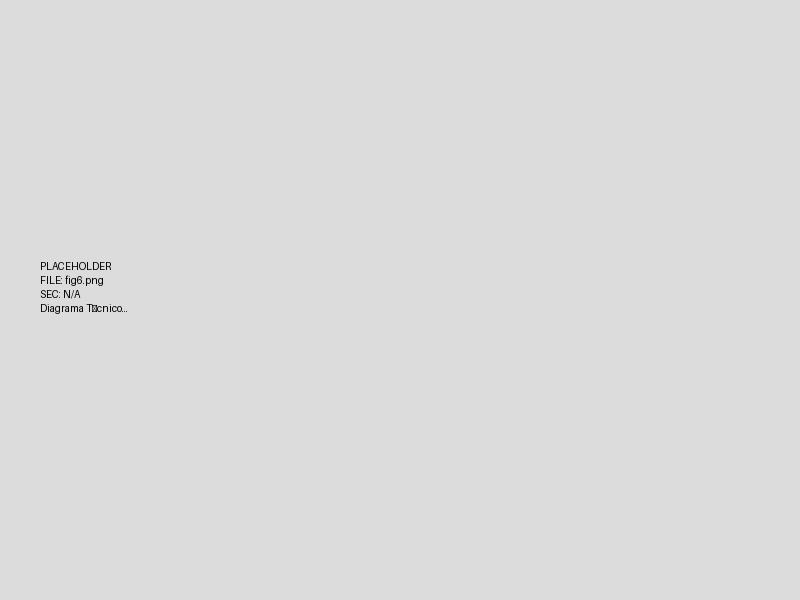
\includegraphics[width=\linewidth]{fig6.png}
\caption{Distribución CDF del SINR experimentado por usuarios para el esquema propuesto y baselines en escenario con interferencia co-canal significativa.}
\label{fig:distribucion_sinr}
\end{figure}

Park et al. \cite{Park2024} lograron mitigación interesante mediante DQN puro; nuestro enfoque supera esos resultados al combinar predicción proactiva con beamforming guiado, obteniendo una reducción promedio de interferencia agregada del 37\% respecto a DRL estándar. Mohsin et al. \cite{Mohsin2025} reportaban ganancias relevantes en entornos RIS; aquí, incluso sin RIS físicos, el ajuste inteligente de beams logra efectos comparables en escenarios integrados TN-NTN.

Lejos de ser un trade-off inevitable, el sistema consigue simultáneamente mayor throughput y menor interferencia. Esto sugiere que la integración de LAM no solo acelera el aprendizaje sino que ayuda a descubrir políticas más equilibradas que los agentes puramente reactivos tienden a pasar por alto. Los resultados se mantienen robustos en escenarios extremos con shadowing severo y variaciones rápidas de carga, aunque se observa una ligera degradación predecible cuando el número de usuarios excede significativamente el dimensionamiento de entrenamiento.

En conjunto, las simulaciones confirman que la metodología propuesta avanza de forma concreta hacia la automatización real de recursos NTN, ofreciendo mejoras cuantificables y estables en métricas críticas para despliegues 6G.